
\section{Aufbau und Durchf"uhrung}
	\label{sec:durchfuehrung}

	Die Abbildung \eqref{aufbau} ist der Aufbau eines Kugelfall-Viskosimeters nach H"oppler.

	\begin{figure}[htbp]
		\centering
		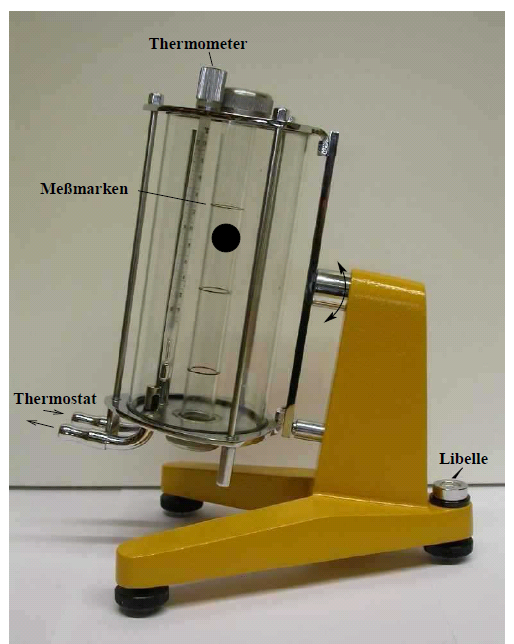
\includegraphics[width = 5cm]{img/aufbau.PNG}
		\caption{Aufbau eines Kugelfall-Viskosimeters nach H"oppler \cite{anleitung}}
		\label{aufbau}
	\end{figure}

	Es steht eine kleine und eine gro"se Glaskugel zur Verf"ugung.
	Zun"achst wird die Dichte der Kugeln aus der Masse und dem Volumen bestimmt.
	Anschlie"send wird das Viskosimeter mit Hilfe der Libelle justiert.
	Das Glasrohr in der Mitte wird m"oglichst frei von Luftblasen mit destilliertem Wasser und jeweils einer der Glaskugeln gef"ullt. 
	Dabei ist die Apparatur um wenige Grad geneigt, damit die Kugel auf dem Wasserfilm gleitet und nicht un\-kon\-trol\-liert an die Wand st"o"st und sich so keine Wirbel ausbilden.
	\\
	Die Fallzeit $t$ der beiden Kugeln wird auf einer Strecke von $\SI{10}{\centi\meter}$ 10 mal mit einer Stoppuhr gemessen, indem die Apparatur nach einem Durchlauf um $180^\circ$ gedreht wird.
	Dabei ist darauf zu achten, dass die Kugel beim Durchlaufen der ersten Messmarke bereits eine konstante Geschwindigkeit erreicht hat.
	Mit gegebenem $K_{\mathrm{klein}}$ kann die konstante Viskosit"at bei Raumtemperatur berechnet werden und daraus die Ap\-pa\-ra\-tur\-kon\-stan\-te $K_{\mathrm{gro"s}}$.
	\\
	Um die R"ohre mit der Kugel befindet sich ein Wasserbad, welches mit einer Heiz\-vor\-rich\-tung verbunden ist.
	Dieses wird nun auf bis zu $55^\circ$C. geheizt und dabei bei 10 verschiedenen Temperaturen je zwei Messungen mit der gro"sen Kugel durchgef"uhrt.